% !TEX root = ../om_ts_002.tex

\begin{frame} % название фрагмента

\videotitle{Stationary processes}

\end{frame}



\begin{frame}{Stationary processes: Plan}
  \begin{itemize}[<+->]
    \item Definition
    \item Random walk 
    \item Autocovariance function
    \item ACF, PACF
    
  \end{itemize}

\end{frame}

\begin{frame}
  \frametitle{Stationary processes}

   A stochastic process whose characteristics \alert{do not change over time}
  \pause

  \begin{block}{Weak or wide-sense stationarity}
    A process $(y_t)$  is said to be   \alert{weakly stationary}, if for each $t$ and $k$:
    \[
    \begin{cases}
      \E(y_t ) = \mu \\
      \Cov(y_t, y_{t+k}) = \gamma_k \\          
    \end{cases}
    \]
  \end{block}

  \pause
  \begin{block}{Strong or strict-sense stationarity}
    A process $(y_t)$  is said to be   \alert{ strictly stationary}, if for each  $k$ 
    joint  distribution of a r.v.  $(y_t, y_{t+1}, y_{t+2}, \ldots, y_{t+k})$ does not depend on  $t$
  \end{block}
\end{frame}




\begin{frame}
	\frametitle{Stationary process: example}
	
	\begin{block}{Independent observations}
		The quantities $(y_t)$ are independent and equally distributed
		with finite expectation $\mu_y$ and finite variance $\sigma^2_y$
	\end{block}
	
	\pause
	\[
	\mu_y = \E(y_t)
	\]
	\pause
	\[
	\gamma_0 = \Cov(y_t, y_t) = \Var(y_t) = \sigma^2_y
	\]
	\pause
	\[
	\gamma_k = \Cov(y_t, y_{t+k}) = 0, \text{ for } k \geq 1
	\]
\end{frame}



\begin{frame}
	\frametitle{Non-Stationary Process Example}
	
	\begin{block}{Random Walk}
		\[
		\begin{cases}
			y_0 = \mu \\
			y_t = y_{t-1} + u_t, \text{ for } t \geq 1 \\
		\end{cases},
		\]
		where $u_t$ is white noise
	\end{block}
	
	\pause
	
	\centering
	
	Explicitly: $y_t = \mu + u_1 + u_2 + \ldots + u_t$.
	\pause
	\[
	\mu_y = \E(y_t)
	\]
	\pause
	\[
	\gamma_0 = \Cov(y_t, y_t) = \Var(y_t) = \Var(\mu + u_1 + \ldots + u_t) = t\sigma^2_u
	\]
	\pause
	\[
	\gamma_k = \Cov(y_t, y_{t+k}) = \Cov(y_t, y_t + u_{t+1} + \ldots + u_{t+k}) = \Var(y_t)
	\]
\end{frame}

\begin{frame}
	\frametitle{Random Walk vs Random Sample}
	
	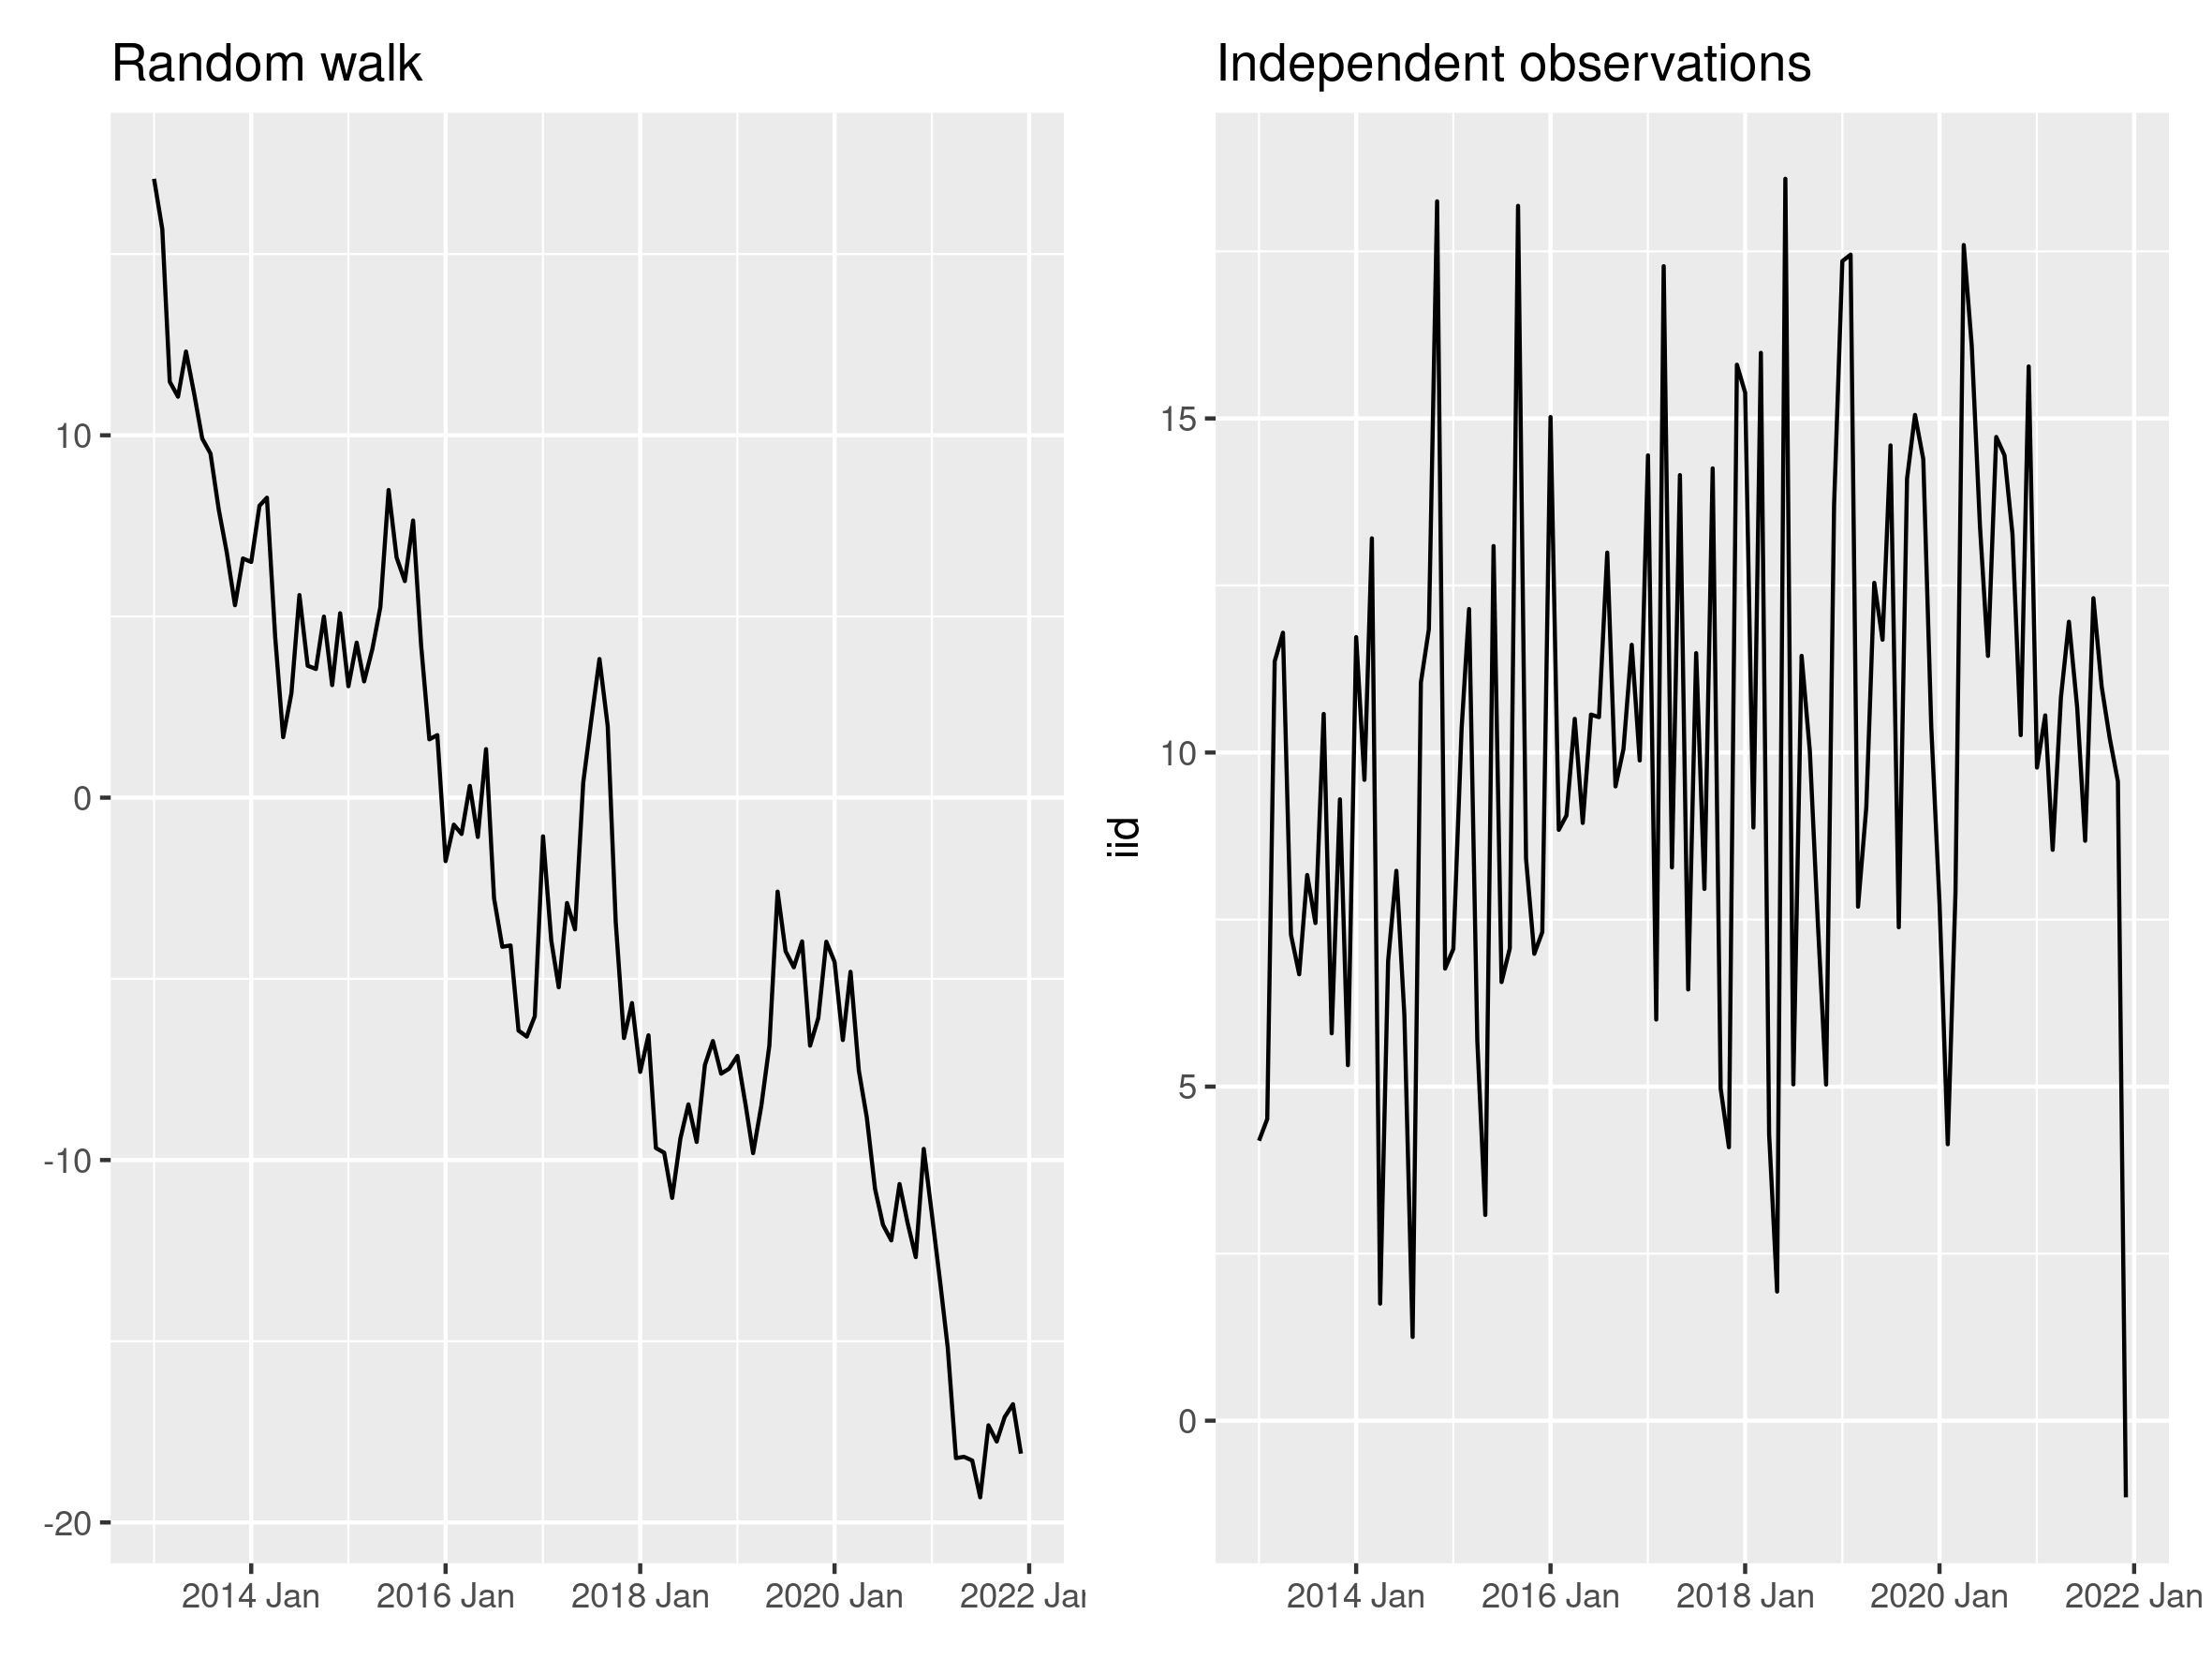
\includegraphics[width=\textwidth]{pictures/om_ts_04-028.png}
	
	
\end{frame}









\begin{frame}
	\frametitle{Autocovariance function}
	
	\begin{block}{Definition}
		For a stationary process $(y_t)$, the function $\gamma_k = \Cov(y_t, y_{t+k})$
		is called \alert{autocovariance}
	\end{block}
	
	\pause
	\begin{block}{Definition}
		For a stationary process $(y_t)$, the function $\rho_k = \Corr(y_t, y_{t+k})$
		is called \alert{autocorrelation}
	\end{block}
\end{frame}



\begin{frame}
\frametitle{ACF: autocorrelation function}
	
	\[
	\rho_k = \Corr(y_t, y_{y+j}) = \frac{\Cov(y_t, y_{y+j})}{\sqrt{\Var(y_t)\Var(y_{t+k})}} =  \pause
	\frac{\gamma_k}{\sqrt{\gamma_0 \gamma_0 }} = \frac{\gamma_k}{\gamma_0}
	\]  
	
\end{frame}




\begin{frame}
	\frametitle{Partial Correlation}
	
	\begin{block}{Definition}
		
		\[
		\pCorr(U, D ; R_1, R_2, \ldots, R_n) = \Corr(U^*, D^*), \text{ where} 
		\]
		\[
		U^* = U - Best(U; R_1, R_2, \ldots, R_n), 
		\]
		\[
		D^* = D - Best(D; R_1, R_2, \ldots, R_n)
		\]    
	\end{block}
	
	\pause
	The values ​​$U^*$ and $D^*$ are the versions of $U$ and $D$ \alert{uninfluenced}  by the covariates $R_1, \ldots, R_n$
	
	\[
	\Cov(U^*, R_i) = 0, \quad \Cov(D^*, R_i) = 0.
	\]
	
\end{frame}


	
	\begin{frame}
		\frametitle{PACF}
		
		\begin{block}{Definition}
			For a stationary process $(y_t)$ the function
			\[
			\varphi_{kk} = \pCorr(y_t, y_{t+k}; y_{t+1}, \ldots, y_{t+k-1})
			\]
			is called \alert{partial autocorrelation}
		\end{block}
	\end{frame}
	
	\begin{frame}
		\frametitle{ACF and PACF: Intuition}
		
		For \alert{stationary process}
		
		\begin{itemize}
			\item ACF:
			\[
			\rho_k = \Corr(y_t, y_{t+k})
			\]
			\alert{Joint strength} of relationship between $y_t$ and $y_{t+k}$
			\item PACF:
			\[
			\varphi_{kk} = \pCorr(y_t, y_{t+k}; y_{t+1}, \ldots, y_{t+k-1})
			\]
			\alert{Strength} of relationship  between  $y_t$ and $y_{t+k}$ with the links through intermediate observations being  \alert{broken}
		\end{itemize}
	\end{frame}
	
	
	
		
	\begin{frame}{Stationary processes: Summary}
		
		\begin{itemize}[<+->]
			\item Constants $\E(y_t)$, $\gamma_k = \Cov(y_t, y_{t+k})$
			\item The random sample is stationary
			\item Random walk is non-stationary
			\item \alert{Autocovariance} function
			\item Partial correlation — correlation with the effect of a set of controlling random variables removed
			\item In the time series, we removed the effect of \alert{intermediate} observations
			
			
		\end{itemize}
		
	\end{frame}
	
	
